%%
%% This is file `example-1.tex',
%% generated with the docstrip utility.
%%
%% The original source files were:
%%
%% drexel-thesis.dtx  (with options: `example-part')
%% 
%% This is a generated file.
%% 
%% Copyright (C) 2010 W. Trevor King
%% 
%% This file may be distributed and/or modified under the conditions of
%% the LaTeX Project Public License, either version 1.3 of this license
%% or (at your option) any later version.  The latest version of this
%% license is in:
%% 
%%    http://www.latex-project.org/lppl.txt
%% 
%% and version 1.3 or later is part of all distributions of LaTeX version
%% 2003/06/01 or later.
%% 

\chapter{Quasi 2-D and 2.5-D Systems}
Studies of traveling waves have focused on two-dimensional waves that spread parallel to the surface (pia) of the brain \citep{reimer2010}\citep{keane2015}\citep{Townsend2018}\citep{Golomb1997}\citep{Qi2015}. 
This is to be expected as this is the geometry of the system on which they are observed, and \citet{Wilson1973} provide an anatomical argument for focusing on such structure. 

We now extend our study of traveling waves in quasi 1-D minicolumns to two-dimensional topologies.
First we study two-dimensional sheets of neurons extended in the X and Y directions.
As before, we find that our model doesn't support traveling waves in a purely two-dimensional sheet (Z=1) under the model parameters studied.
When we extend the system to a quasi two-dimensional sheet (Z=2) we find traveling waves are evoked by both the background and impulsive stimulus.
Our model exhibits the same categories of two-dimensional waves observed in the brain.

We then further extend our topology to what we term a ``forest'' of minicolumns.
This structure consists of an ensemble of our minicolumns arranged on a grid, with the Z extent less than the X/Y extents.
We find that our forest supports transverse traveling waves in the X/Y plane.

\section{Two-dimensional sheets of neurons}
Traveling waves in two-dimensional neuronal sheets have been studied in the brain \citep{huang2004}\citep{Townsend2018} and in simulation\citep{keane2015}\citep{Spreizer2019}
While one-dimensional waves have only one structure, the additional degree of freedom in two dimensions allows for several categories of waves.
These include circular waves that spread outward from a point, large plane waves that propagate over the entire surface and spiral waves\citep{Huang2010}\citep{Gu2013} that rotate around a phase singularity.
Different types of waves have been associated with different elements of visual stimulus\citep{Benucci2007}.
We find evidence for all these categories of waves in our quasi two-dimensional sheet.

Each sheet consists of neurons placed on a unit grid. 
The X and Y extents are much larger than the Z extent.
We generally use sheets with Z=2 with the exception of one purely two-dimensional example with Z=1.
Neurons are created and connected as described in Methods.
Due to the larger area of regard and the more demanding computational experiments we use periodic boundary conditions in our quasi two-dimensional sheets.
A small example quasi 2-D sheet is shown in Figure \ref{fig:sheet_structure}.
In this small example the periodic boundary conditions are easily seen as multiple diagonals in the connection matrix.

\begin{figure}[!htb]
 \caption{Example small quasi 2-D sheet with dimensions X=10, Y=10, Z=2. The connection parameters are set to $\lambda$=2.5 and C=0.5. 
 a)  Sheet showing connections between neurons as lines colored using a color scale that indicates the connection length. 
 b)  Connection matrix. E-E connections are green, E-I are black and both I-E and I-I  are red. 
 c) The sum of presynaptic weights for each neuron shows the anisotropy of this model, with substantial variation in input strength and sign between the neuron inputs.}
 \label{fig:sheet_structure}
 \subfloat[][]{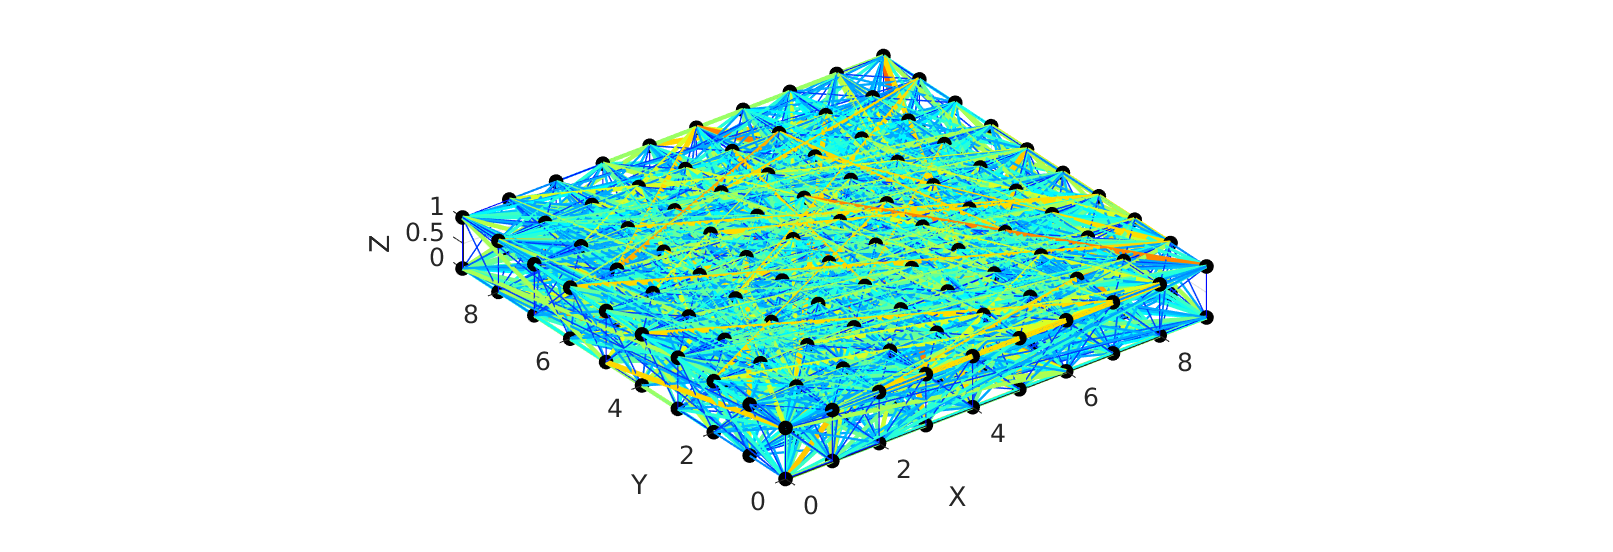
\includegraphics[width=\textwidth]{fig/Sheet_Structure_A}}
 \subfloat[][]{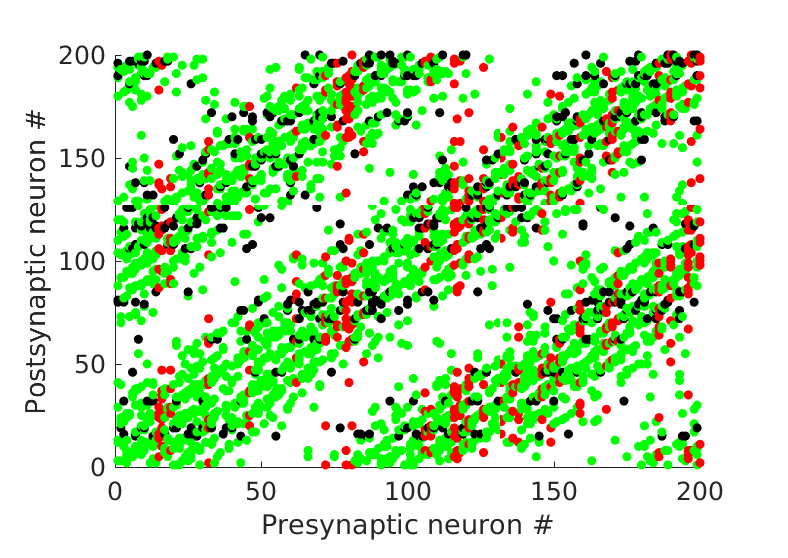
\includegraphics[width=0.4\textwidth]{fig/Sheet_Structure_B}}
 \subfloat[][]{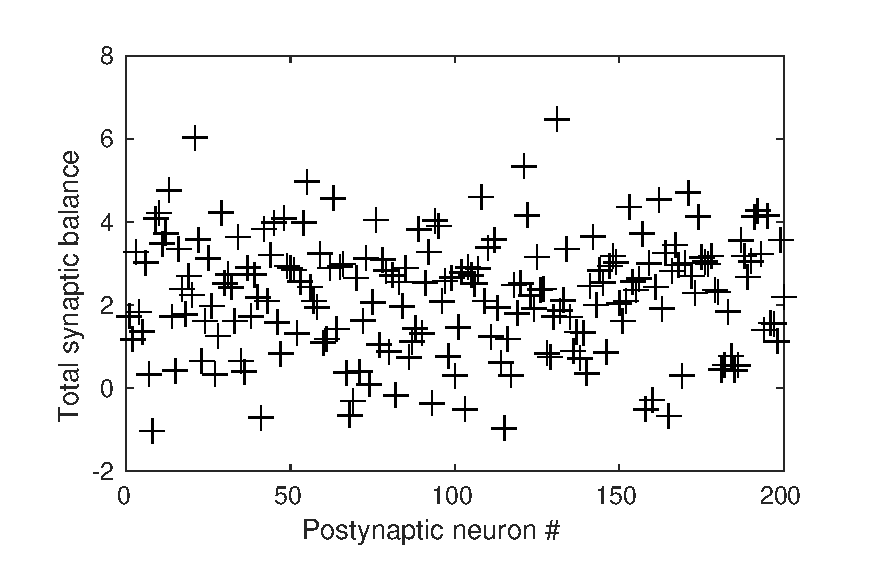
\includegraphics[width=0.4\textwidth]{fig/Sheet_Structure_C}}
\end{figure}

The topology of our sheet combined with our local connectivity rule (eq. \ref{eq:connectivity}) defines the connection distribution of the sheet.
The distribution of post-synaptic connections and delay times are shown in Figure \ref{fig:connection_delay_distrbution_2D} for an example quasi 2-D sheet.
Compared the to minicolumn connection distribution in figure \ref{fig:connection_delay_distrbution} the neurons in our sheet have on average about twice as many connections.
The length of the connections between neurons tends to be longer in the sheet, resulting in a distribution of longer delays 
in figure \ref{fig:connection_delay_distrbution_2D} when compared to figure \ref{fig:connection_delay_distrbution}.
\begin{figure}[!htb]
 \caption{Distribution of (a) number of post-synaptic connections per neuron and (b) delay time. 
          Data was taken from an X=100, Y=100, Z=2 sheet with $\lambda=2.5$, $\kappa=1$ and periodic boundary conditions.  } 
     \subfloat[][]{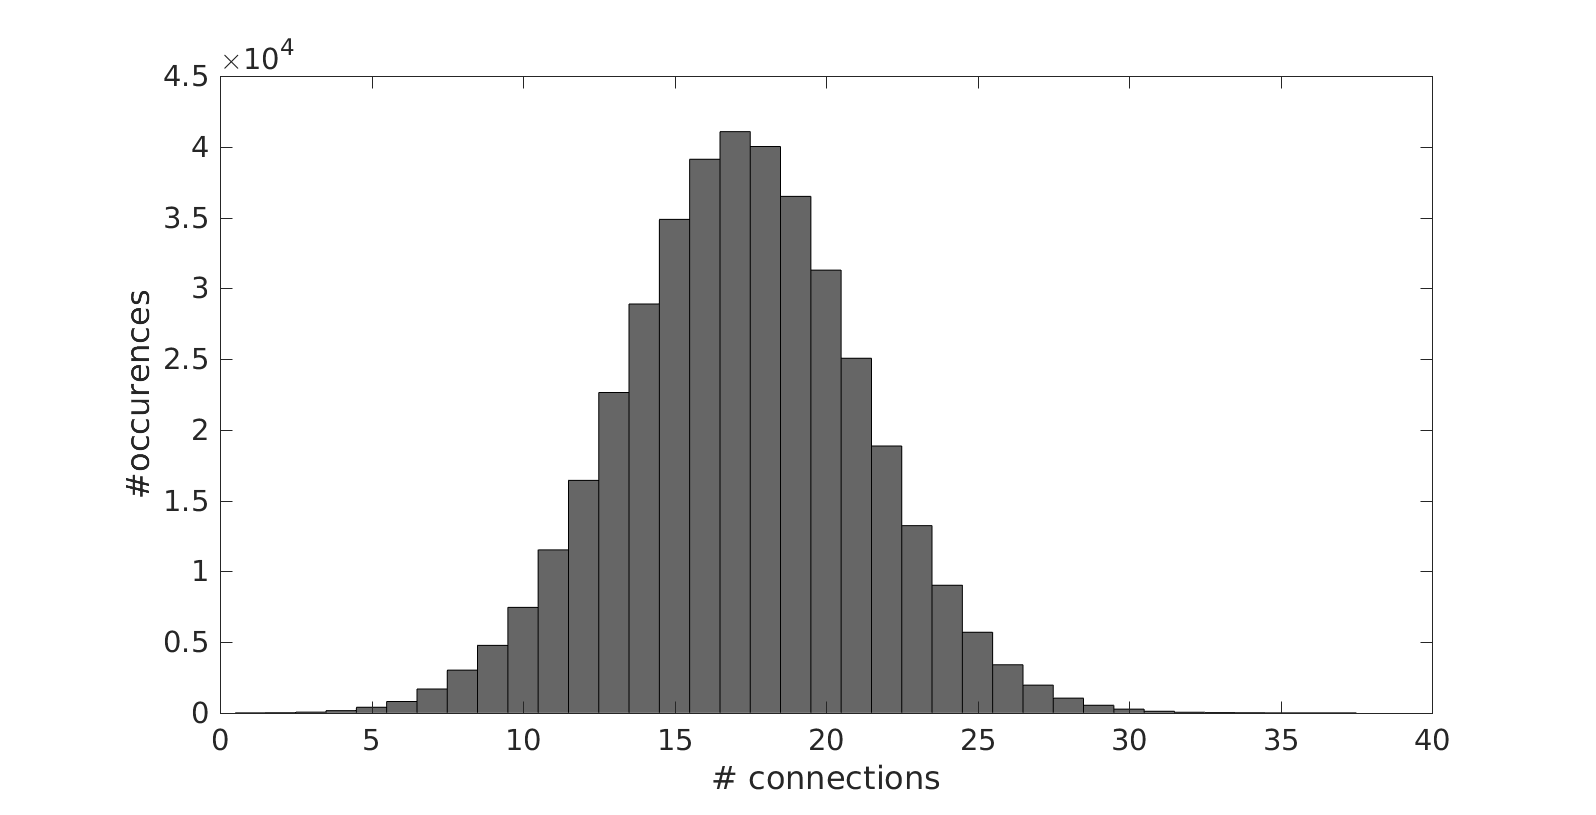
\includegraphics[width=0.6\textwidth]{fig/ConnectionNumberDistribution2D} }
     \subfloat[][]{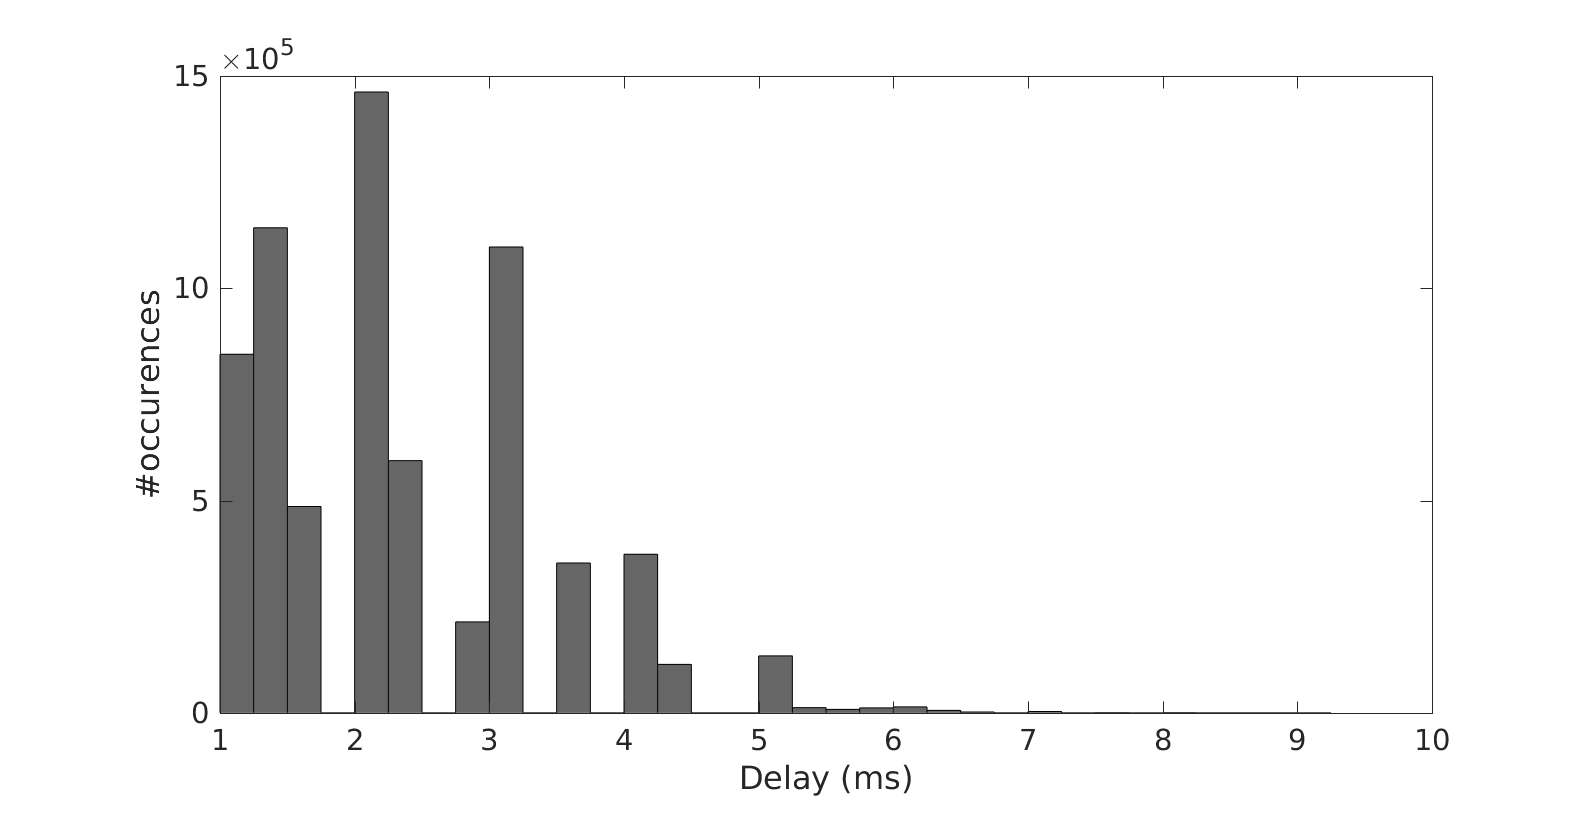
\includegraphics[width=0.6\textwidth]{fig/DelayDistribution2D} }
 \label{fig:connection_delay_distrbution_2D}
\end{figure}
 \FloatBarrier

As we did with our quasi 1-D minicolumn, we first create a purely 2-D sheet of neurons with X=100, Y=100 and Z=1.
Model parameters are fixed at $\Sigma$.
We do not observe traveling waves or other spatiotemporal patterns in this system (Figure \ref{fig:Pure2DRasters_NoWaves}).
\begin{figure}[!htb]
 \caption{ Raster plots from our purely 2-D system do not show coherent spatiotemporal patterns.}
 \label{fig:Pure2DRasters_NoWaves}
 \centering
   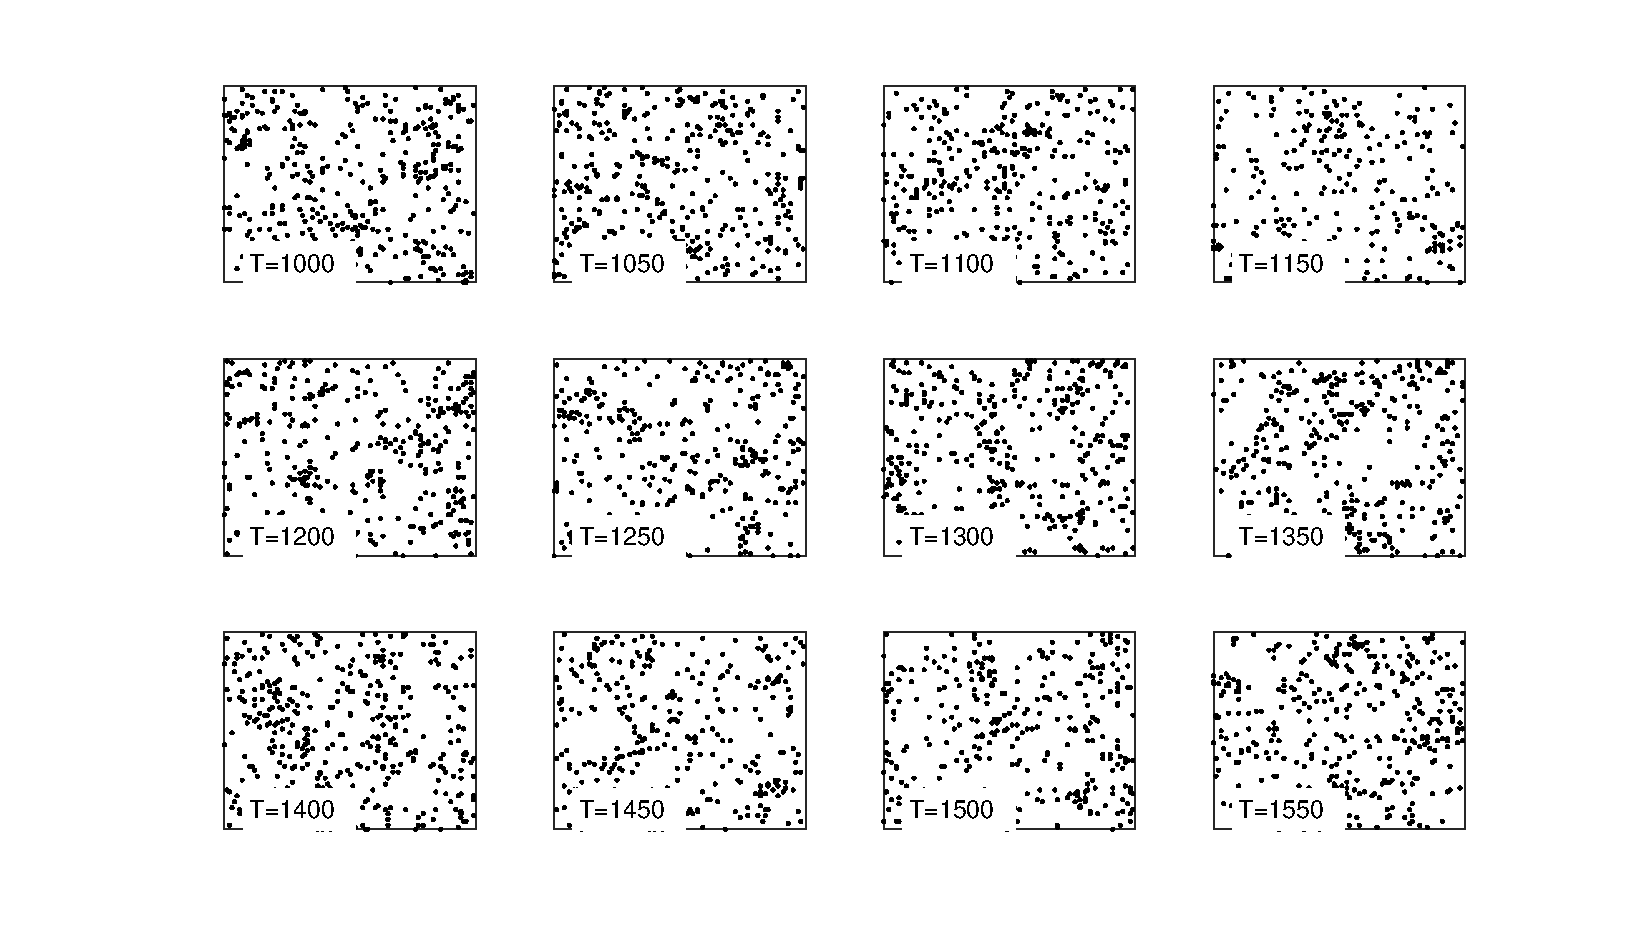
\includegraphics[width=\textwidth]{fig/2DWaveRasters_1LayerNoWaves}
\end{figure}
\FloatBarrier

We then extend our system to a quasi 2-D sheet with X=200, Y=200 and Z=2.
We now observe traveling wave patterns in the system.
These patterns emerge in spite of the high variability in the neuron types, neuron dynamics and connectivity present in our model.
We can clearly see  circular spreading waves emanating from multiple points within the sheet \ref{fig:2D_waves}.
These types of spreading waves have been observed in vivo\citep{Mohajerani2013} and and in vitro, and can be spontaneously generated or evoked by a stimulus\citep{Stroh2013}.
\begin{figure}[!htb]
 \caption{ Wave patterns spreading across the surface of a sheet. 
           the sheet dimensions are 200x200x2, model parameters are at $\Sigma$. 
           Circular spreading waves are the dominant type, but multiple waves can interact to form more complex patterns.}
 \label{fig:2D_waves}
 \centering
   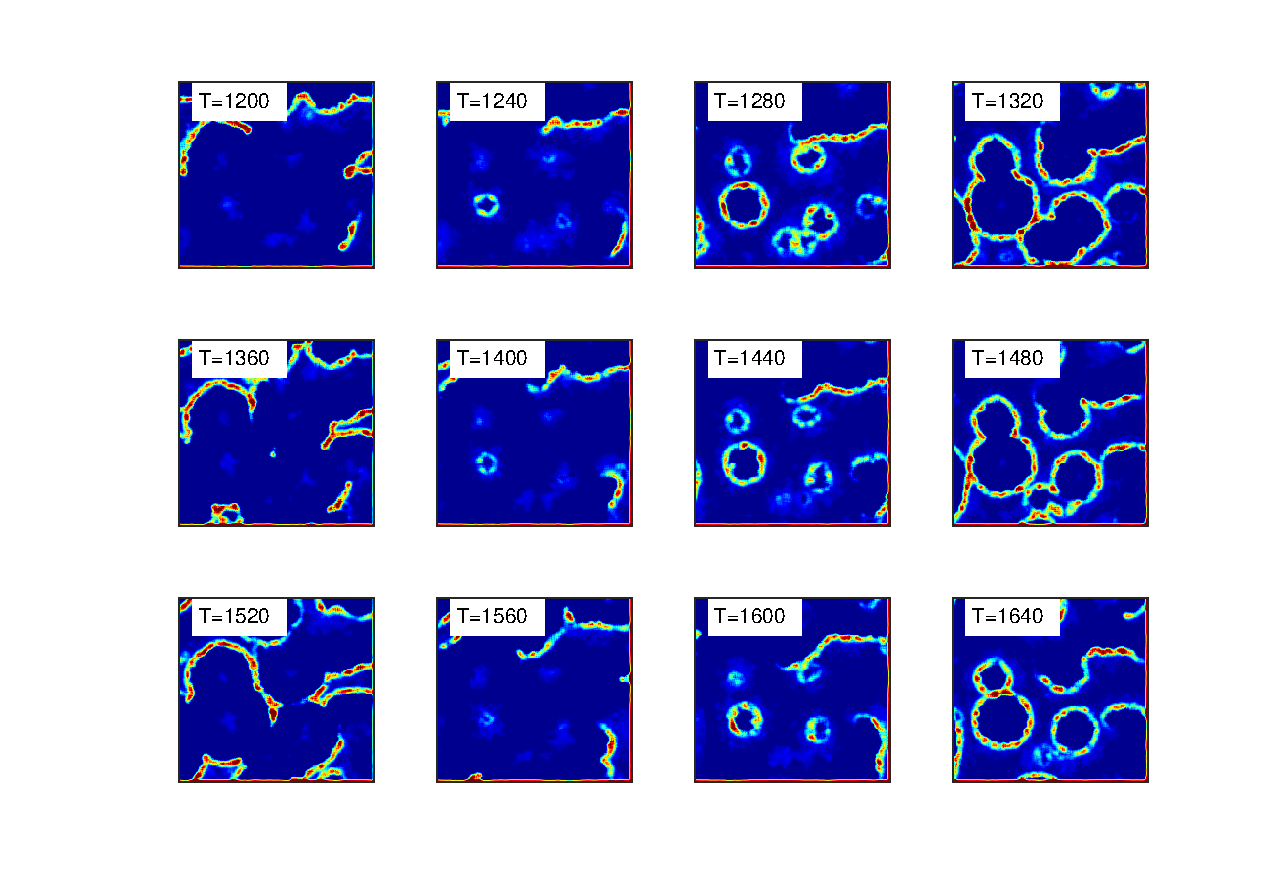
\includegraphics[width=\textwidth]{fig/2DSpreadingWaves_Sigma}
\end{figure}

\FloatBarrier

In some simulations we see the formation of large-scale plane waves across the entire system as seen by \citet{keane2015}.
In their work, plane waves were formed when excitation dominated their neuronal system.
These plane waves seem to form due to the interaction of spreading circular waves.
The formation of plane waves in our system does not seem deterministic, as a different random draw of the uniform background stimulus for the same neuronal system may not exhibit plane waves.
Nonetheless, these results show that plane waves can emerge as a stable pattern in systems of this type even when excitation does not dominate.
\begin{figure}[!htb]
 \caption{ A plane wave front forming from multiple circular spreading waves.
          The sheet is 200x200x2, model parameters are at $\Sigma$.}
 \label{fig:2D_plane_wave}
 \centering
   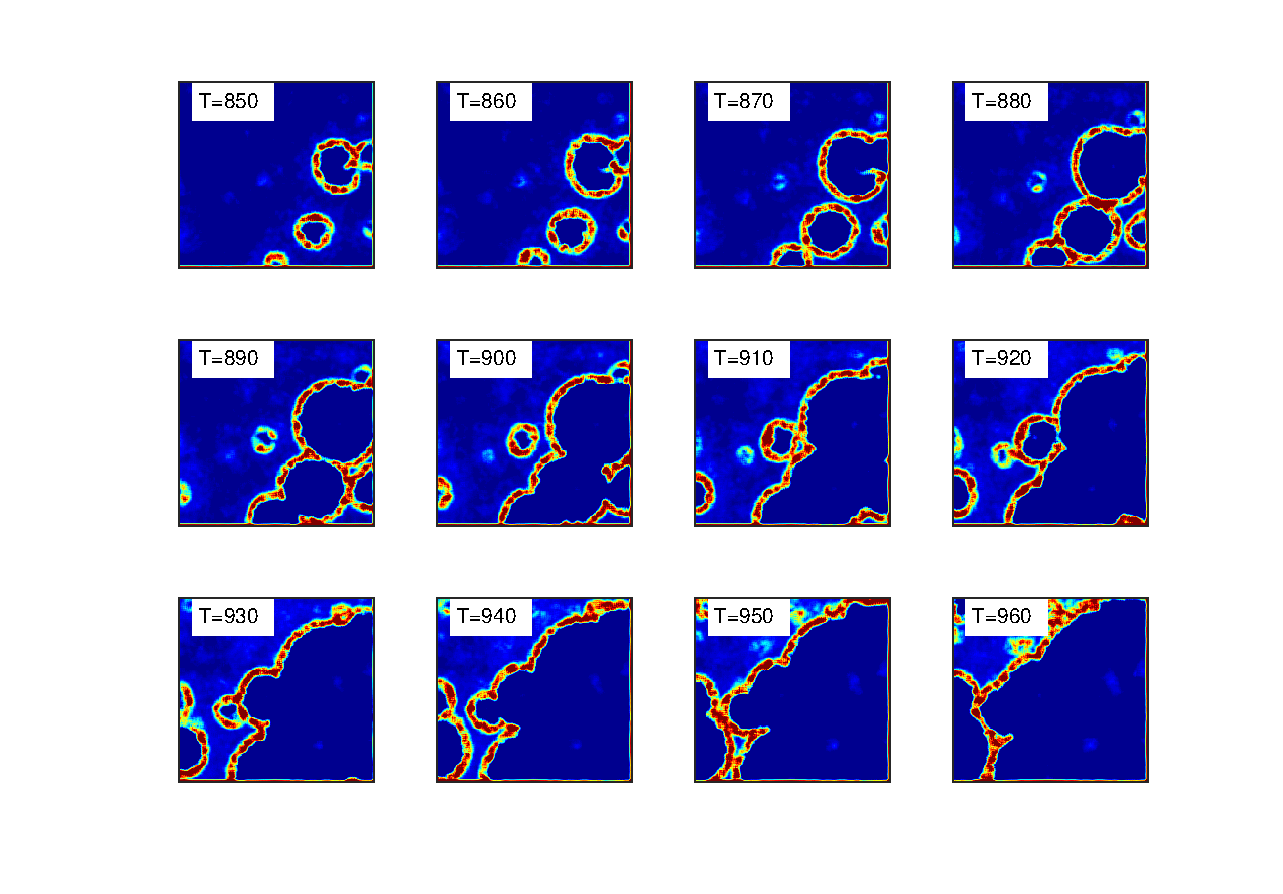
\includegraphics[width=\textwidth]{fig/2DPlaneWave}
\end{figure}
\FloatBarrier

When the wave speed increases we observe attractor states, where waves spawned from a small number of locations come to dominate the firing activity.
In figure \ref{fig:2DWaveRasters_attractor} we see that the waves spawned from the upper right section of the sheet come to dominate the firing activity.
\begin{figure}[!htb]
 \caption{ Raster plots from our quasi 2-D system showing an attractor forming near X=70,Y=75.}
 \label{fig:2DWaveRasters_attractor}
 \centering
   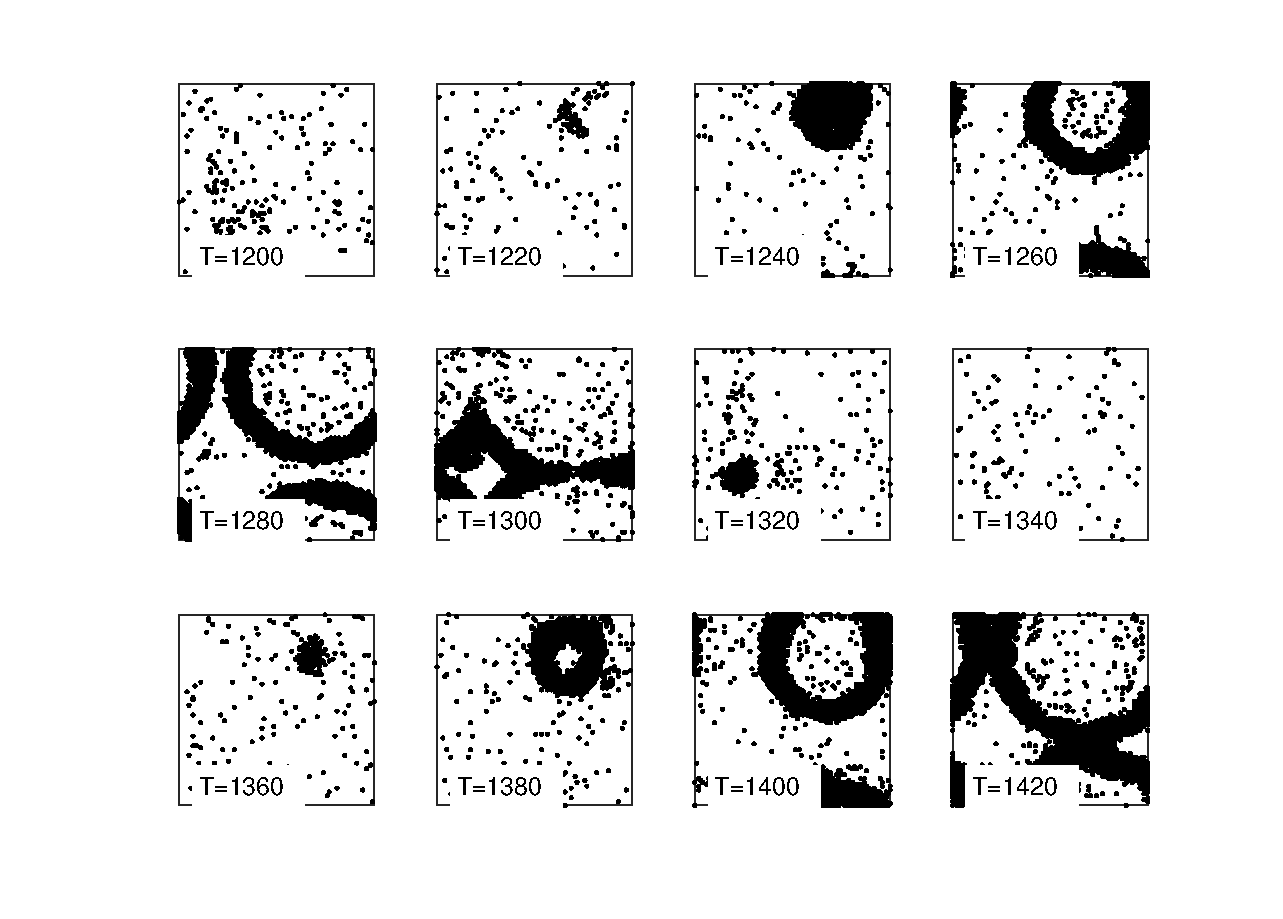
\includegraphics[width=\textwidth]{fig/2DWaveRasters_Attractor_kappa0p1_seed35}
\end{figure}

We do not observe spiral waves in our simulations with the model parameters set at $\Sigma$.
With the higher connectivity observed in the sheet (figure \ref{fig:connection_delay_distrbution_2D}) we see circular waves emanating from a point.
Although these waves can combine to form a plane wave structure (figure \ref{fig:2D_plane_wave}), we have not observed spiral wave patterns.
Given that the sheet has higher connectivity than the minicolumn, we reduce the connection strength K from $K=10$ to $K=6$.
The waves at the lower connection strength are thinner and sparser.
We now observe the formation of spiral wave pattern as seen in figure \ref{fig:2DSpiralWaves}.
\begin{figure}[!htb]
 \caption{ Spiral waves are apparent in the average membrane potential observed in a 2D sheet over time. 
           The sheet is 200x200x2 with periodic boundary conditions, $K=6$, $\kappa=0.1$.
           A 5x5 smoothing filter has been applied. }
 \label{fig:2DSpiralWaves}
 \centering
   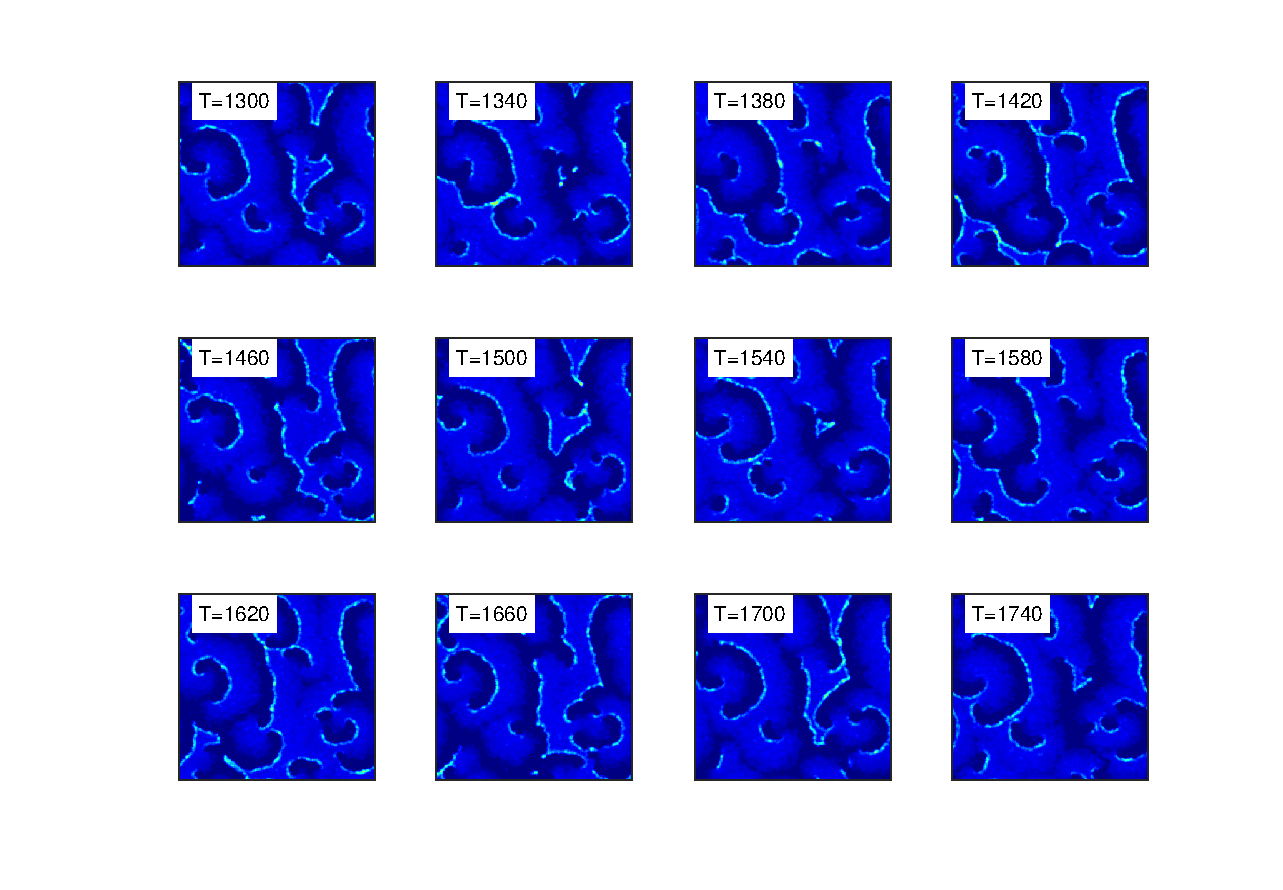
\includegraphics[width=\textwidth]{fig/SpiralWaves2D_K6_kappa0p1_M4}
\end{figure}
\FloatBarrier

\citet{Huang2010} provide the observation that a plane wave with limited extents can generate a spiral wave pattern.
The firing activity at the edge of the plane wave will spread in directions that are not parallel to the plane wave propagation.
We observe similar behavior when the propagation of a circular spreading wave is not isotropic.
In this case we can see spiral waves shed from both edges of the circular wave as seen in figure \ref{fig:2DHeartWaves}.
We term these 'heart' waves.
\begin{figure}[!htb]
 \caption{ Spiral 'heart' waves are apparent in the average membrane potential observed in a 2D sheet over time. 
           The sheet is 200x200x2 with periodic boundary conditions, $K=6$, $\kappa=0.1$.
           A 5x5 smoothing filter has been applied. }
 \label{fig:2DHeartWaves}
 \centering
   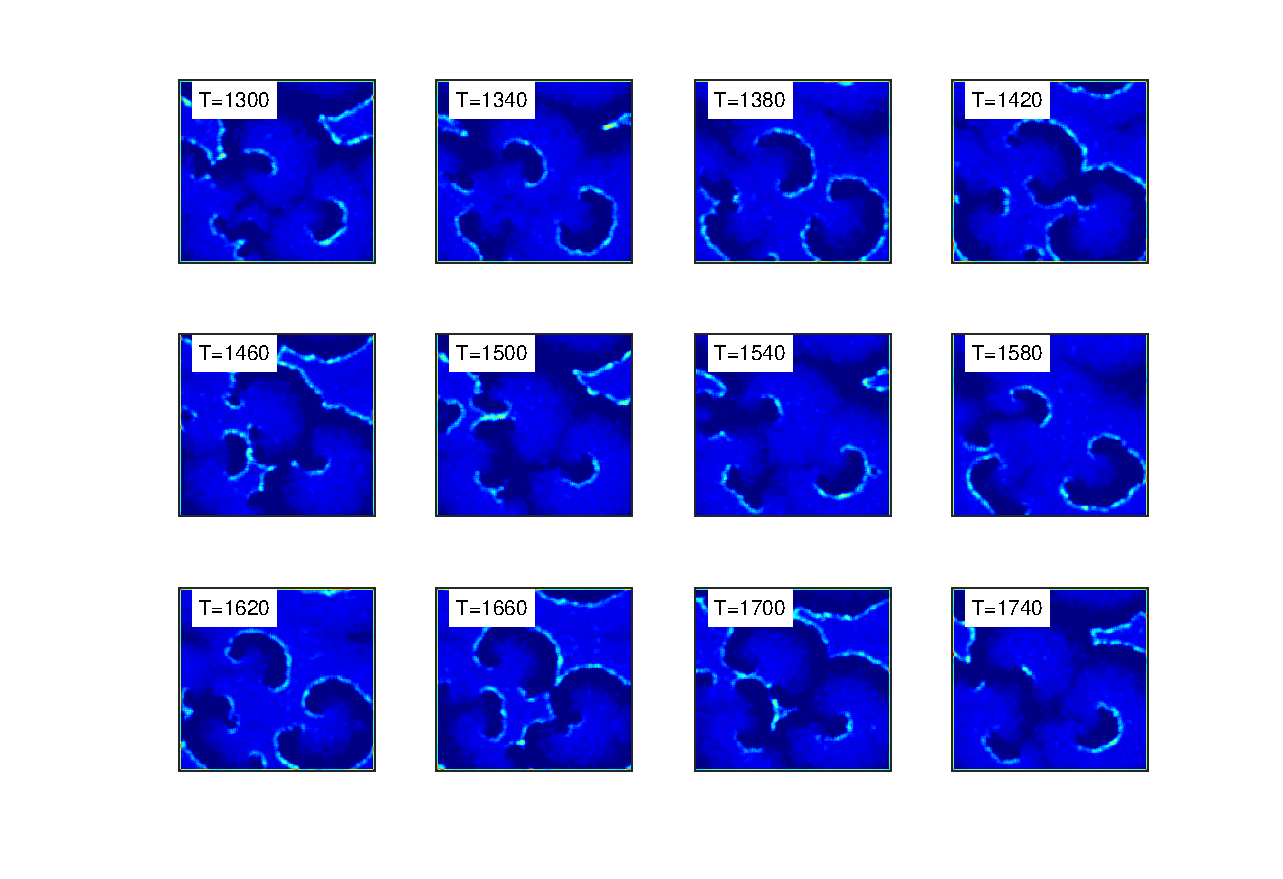
\includegraphics[width=\textwidth]{fig/2DSpiralWaves_HeartWaves}
\end{figure}
\FloatBarrier

We further examine the transition from spreading waves to spiral waves as connection strength decreases.
Our experimental setup is a 100x100x2 sheet with a step stimulus as described in section \ref{sec:wave_speed_method}.
The stimulus is applied to the neurons at the center of the sheet at $t=0$ and generates waves that radiate outward.

We wish to determine whether a given experiment produced a spreading wave or spiral wave.
To distinguish between the wave types we calculate the center of mass of the spikes that occur in a $5~ms$ window:
\begin{align}
 CoM_x &= \frac{1}{N_{spikes}}\Sigma_{i=1}^{N_{spikes}} X_i\\
 CoM_y &= \frac{1}{N_{spikes}}\Sigma_{i=1}^{N_{spikes}} Y_i
\end{align}
where $X$ and $Y$ are the X and Y locations of the spikes w.r.t to center of the sheet, and $N_{spikes}$ is the total number of spikes that occur in the $5~ms$ observation.
We then calculate the center of mass offset as $d_{CoM}=\sqrt{CoM_x^2 + CoM_y^2}$.
The spreading waves have a low $d_{CoM}$ due to their high symmetry, while the spiral waves have a higher $d_{CoM}$.
\begin{figure}[!htb]
 \caption{Transition between spiral and spreading waves as $K$ increases..
          a) Spike raster plot showing a spiral wave in a sheet with $K=9.5$. The center of mass is displaced almost 22 units from the center at $t=100$ indicating the asymmetry of the wave.
          b) Spike raster plot showing a spreading wave in a sheet with $K=10.5$. The center of mass is displaced only 2.5 units due to the high symmetry of the wave.
          c) The system undergoes a transition from asymmetric spiral waves to symmetric spreading waves as the connection strength parameter$K$ increases.
          } 
     \subfloat[][]{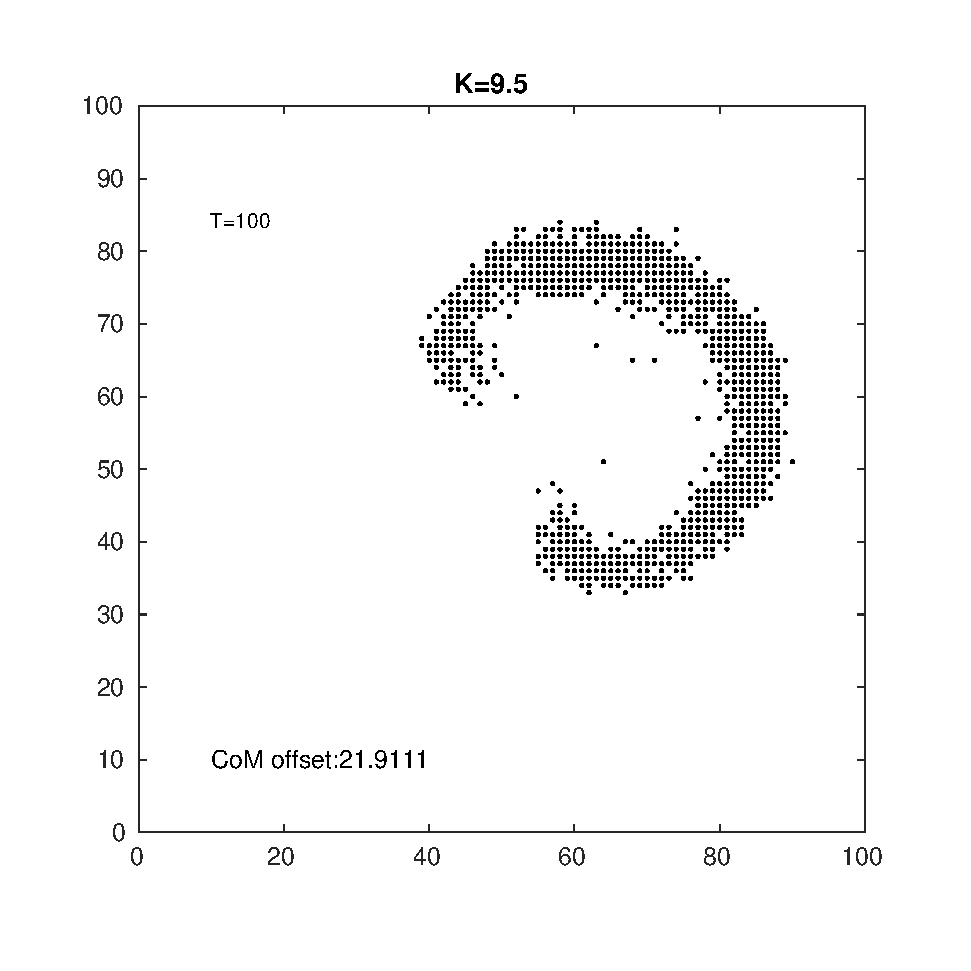
\includegraphics[width=0.45\textwidth]{fig/CoM_Example_K_9p5} }
     \subfloat[][]{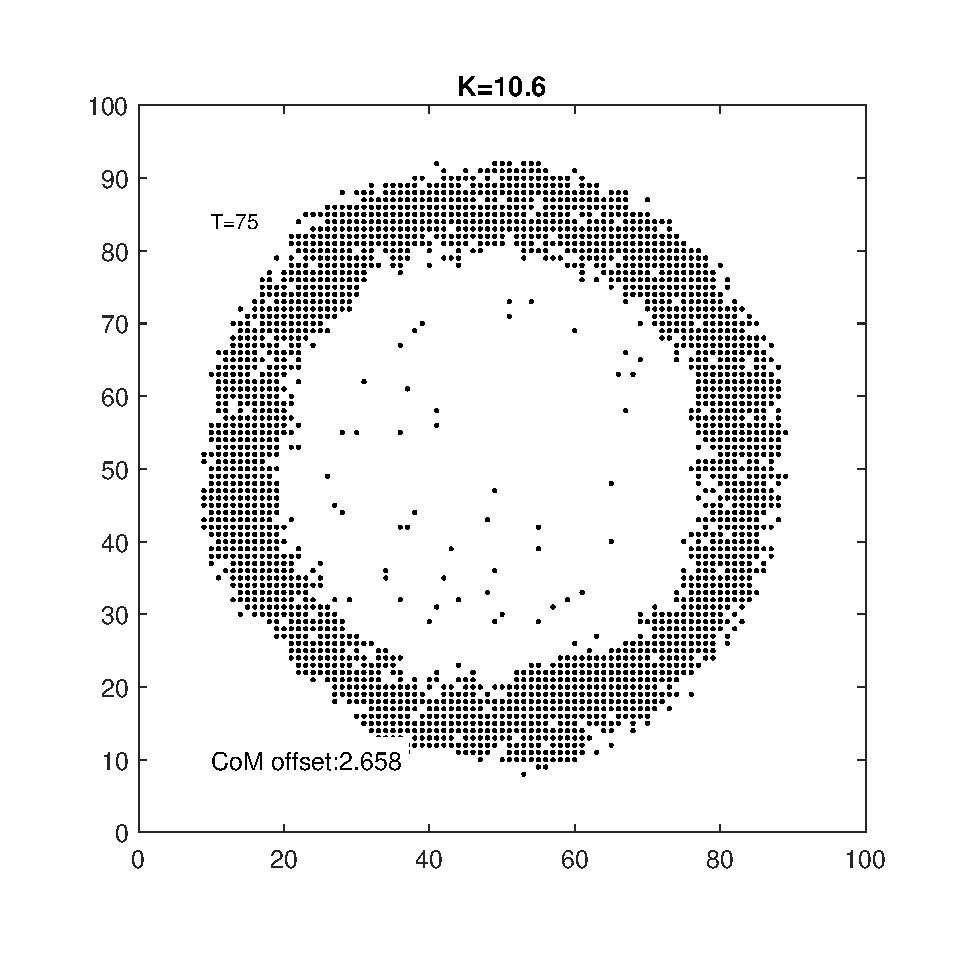
\includegraphics[width=0.45\textwidth]{fig/CoM_Example_K_10p5} }
     \subfloat[][]{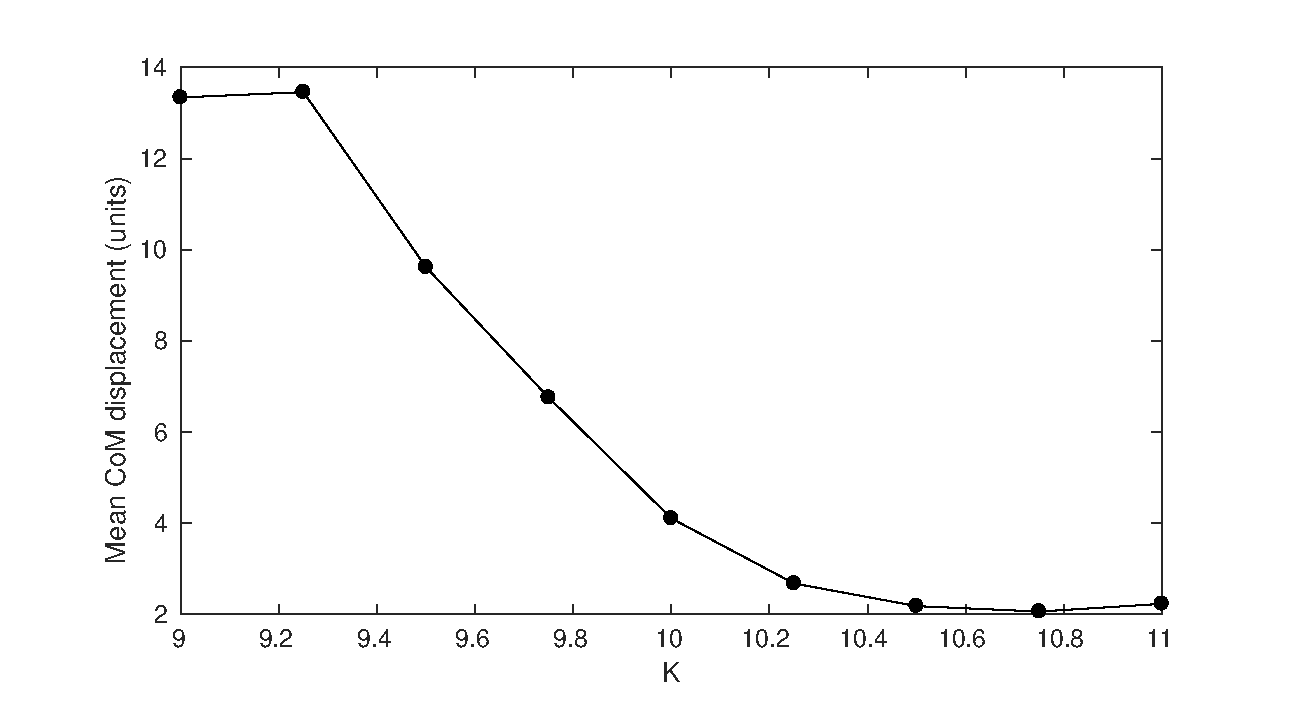
\includegraphics[width=0.75\textwidth]{fig/2DWaveTypeTransition} }
 \label{fig:2DWaveTransition}
\end{figure}
 \FloatBarrier

 In \citet{keane2015} traveling waves in 2-D sheets were proposed to explain why individual spike timing is highly irregular 
but membrane potential fluctuations can be correlated.
We calculate the coefficient of variation of the inter-spike intervals for the spiral wave experiment.
Our overall coefficient of variation is <> indicating highly variable firing in agreement with experimental results.
However, the spike count correlation shows a strong dependence on the distance between neurons.
The traveling waves in our model thus also exhibit strong spike correlations with highly irregular spike times.
\begin{figure}[!htb]
 \caption{Spike timing characterization of the spiral waves seen in figure \ref{fig:2DHeartWaves}.
          a) The spike raster from a small number of neurons show regular spike events that correspond to passing waves.
          b) The distribution of the coefficient of variation confirms the regular spiking behavior as most of the CV values are near 0 (perfectly regular).
          c) The average correlation coefficient as a function of distance shows that the firing times of nearby neurons are highly correlated due to the wave structure.
          } 
     \subfloat[][]{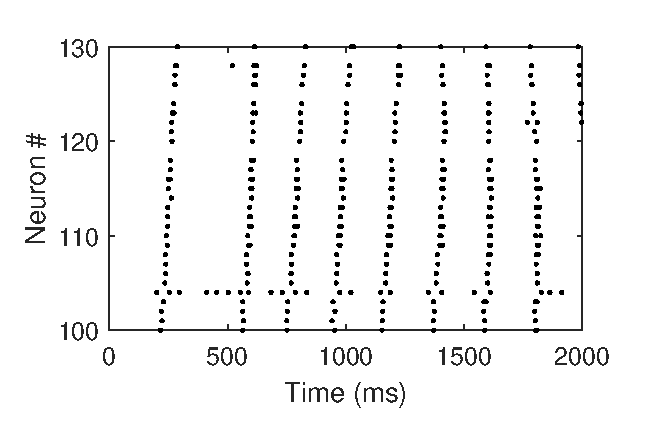
\includegraphics[width=0.4\textwidth]{fig/2DSpiralWaves_CorrelationRasterPlot} }
     \subfloat[][]{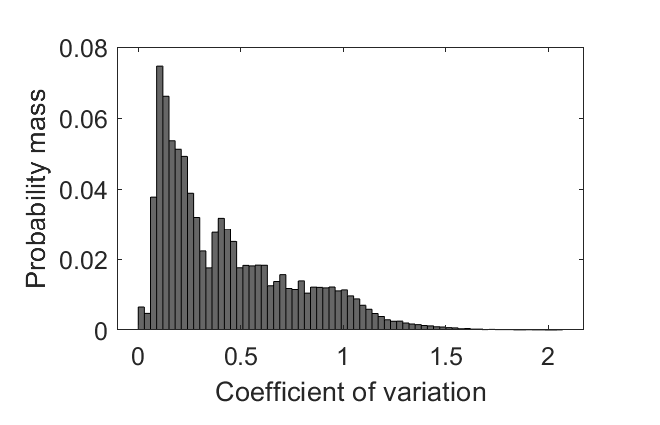
\includegraphics[width=0.4\textwidth]{fig/2DSpiralWaves_CVDist} }
     \subfloat[][]{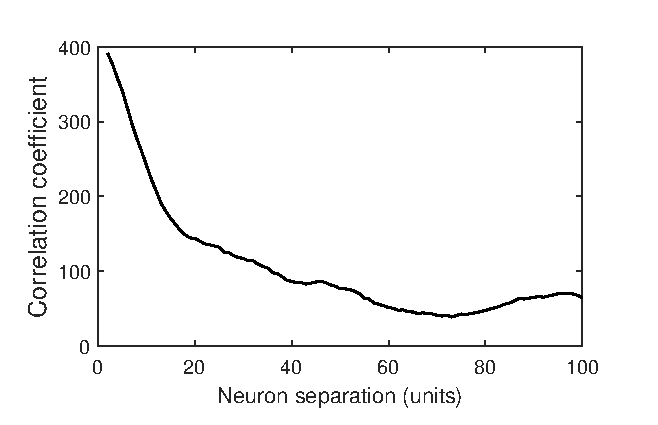
\includegraphics[width=0.4\textwidth]{fig/2DSpiralWaves_CorrelationCoefficient} }
 \label{fig:2DSpiralWave_SpikeTiming}
\end{figure}
 \FloatBarrier
 

The traveling wave mechanism in the locally connected two dimensional sheet is the same as the locally connected one dimensional minicolumn.
We therefore expect similar traveling wave speeds, with the model parameters playing the same role as in the one dimensional minicolumn.
To measure speed in the sheet we extend the approach taken for the minicolumn by using an impulsive stimulus (equation ).
We use open boundary conditions when measuring wave speed in the two dimensional sheet.
We again find that we need to increase the connection strength $K$ when using an impulsive stimulus instead of a uniform background stimulus.
The neurons in the lower left corner near X=0, Y=0 are stimulated with a constant current for the first 10 milliseconds of the simulation.
This induces a circular spreading wave that spans the sheet as shown in figure \ref{fig:2DWaveSpeedRaster}.
The wave propagates isotropically with the same speed along both the X and Y axes.
The wave spans $100$ units in $192~ms$ for a speed of $0.52$ units/millisecond.
This is faster than the measured wave speed of $0.38$ units/millisecond in the minicolumn with the same model parameters.
As seen in figure \ref{fig:delay_topology} increasing the physical extents of our system increases the 
connectivity (figure \ref{fig:connection_delay_distrbution_2D}) leading to faster wave speeds.
\begin{figure}[!htb]
 \caption{ 2-D spike raster plots showing a single traveling wave.
           The sheet is 100x100x2 with model parameters at $\Sigma_v$ and $\kappa=1.0$.
           }
 \label{fig:2DWaveSpeedRaster}
 \centering
   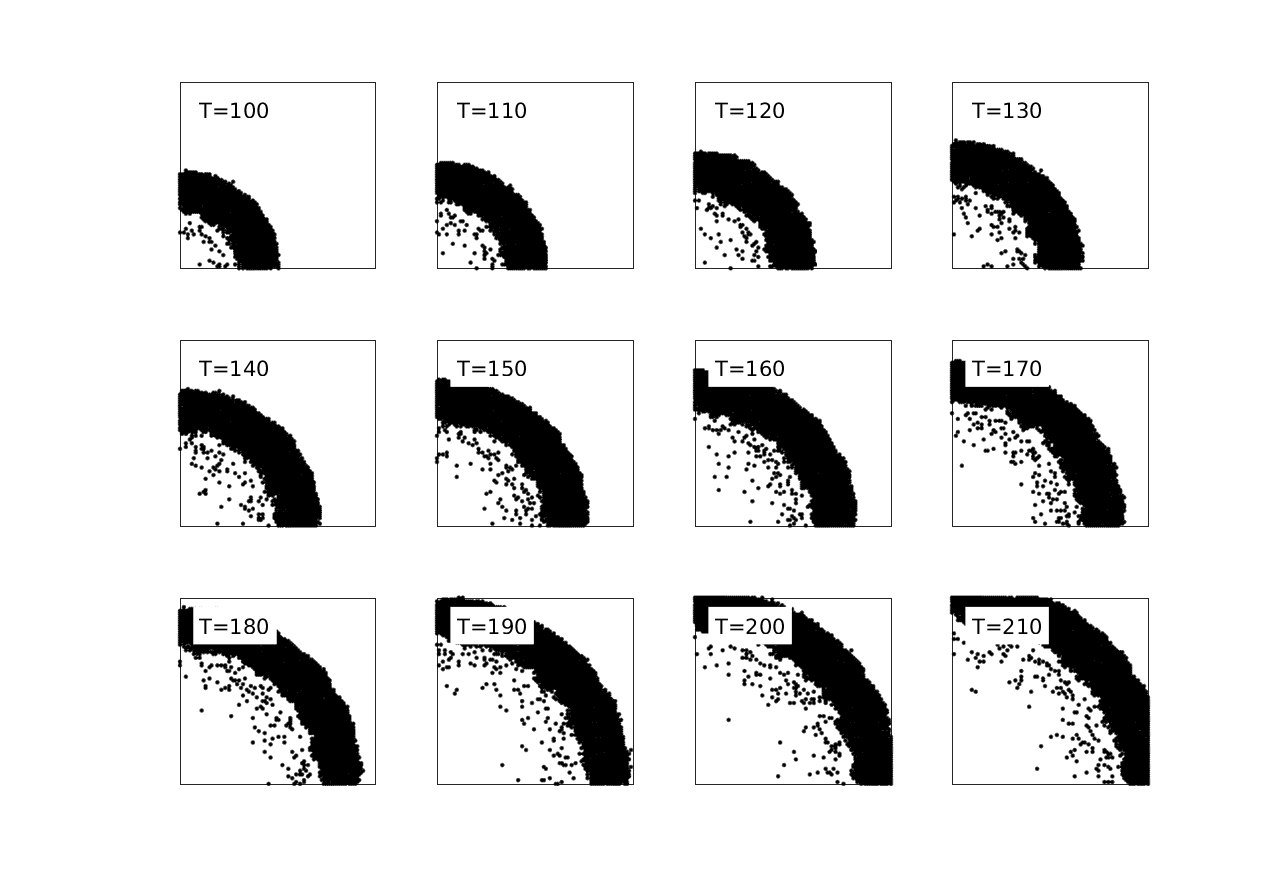
\includegraphics[width=\textwidth]{fig/2DWaveRasters_WaveSpeedExample}
\end{figure}
\FloatBarrier

The wave speed in our sheet depends on $\kappa$ (figure \ref{fig:2DWavePaceKappa}).
The slope of the linear fit matches the one-dimensional system (figure \ref{fig:delay_speed}). 
The lower y-intercept point in the sheet compared to the minicolumn indicates the lower pace (higher speed) due to the higher connectivity in the sheet.
\begin{figure}[!htb]
 \caption{ The pace of the wave depends linearly on $\kappa$.
           }
 \label{fig:2DWavePaceKappa}
 \centering
   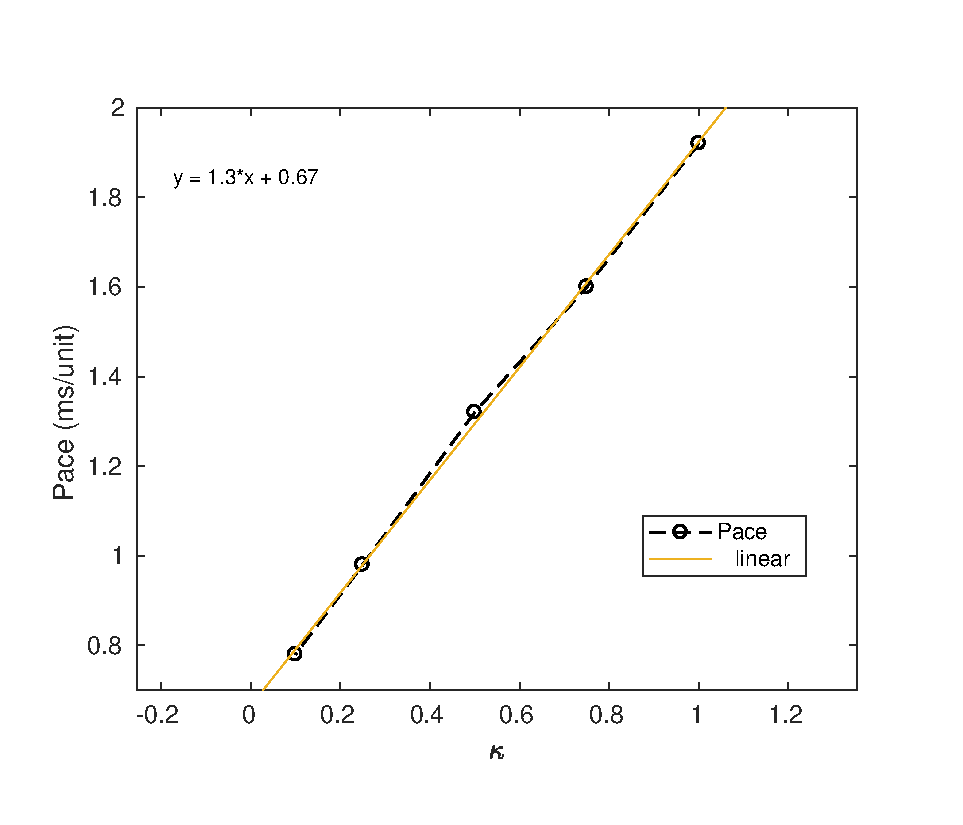
\includegraphics[width=0.5\textwidth]{fig/2DWavePace_Kappa}
\end{figure}
\FloatBarrier


\section{Forests of minicolumns}
The cortex has a laminar vertical organization.
In the visual cortex sponteaneous and stimulus-evoked activity are initiated in different layers\citep{Sakata2009}.
Our forest of minicolumns is an ensemble of 400 or 600 minicolumns arranged in a 20x20 or 30x30 pattern.
Each minicolumn is 2x2x10.
A small example foresst is shown in Figure \ref{fig:forest_structure}.
\begin{figure}[!htb]
 \caption{ Example forest of 16 minicolumns arranged in a 4x4 grid, with $1\lambda$ spacing between the closest neurons of any two minicolumns. 
              Each minicolumn has dimensions X=2, Y=2, Z=5. The connection parameters are $\lambda$=2.5 and C=0.5. 
          a)  Sheet showing connections between neurons as lines colored using a color scale that indicates the connection length. 
          b)  Connection matrix. E-E connections are green, E-I are black and both I-E and I-I  are red. }
 \label{fig:forest_structure}
 \subfloat[][]{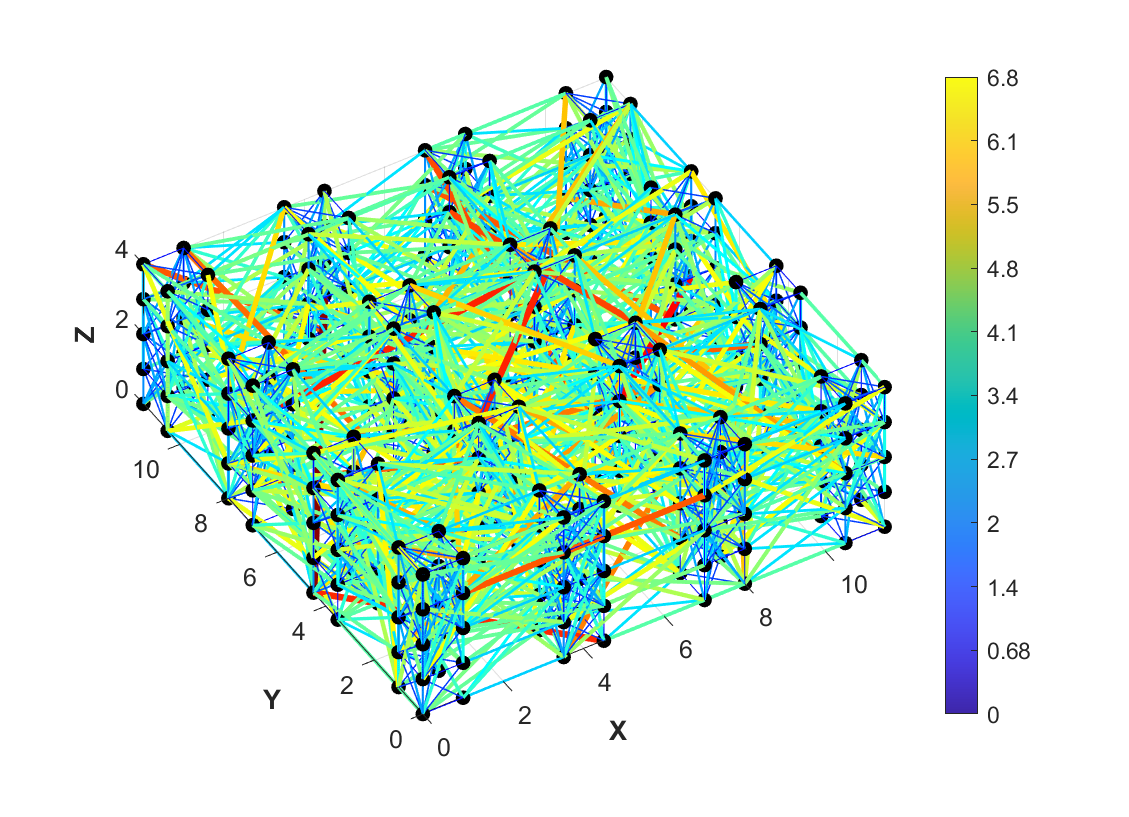
\includegraphics[width=0.75\textwidth]{fig/Forest_Structure_A}}
 \subfloat[][]{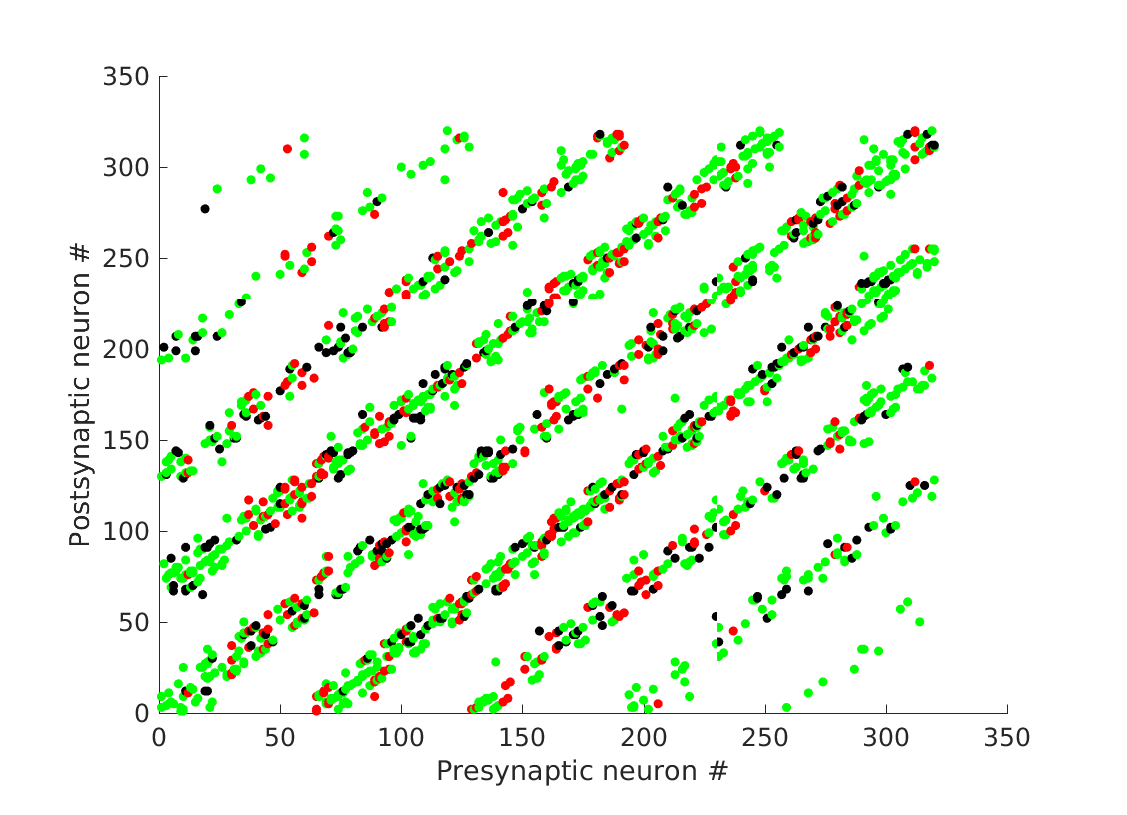
\includegraphics[width=0.75\textwidth]{fig/Forest_Structure_B}}
\end{figure}
\FloatBarrier

We wish to compare the overall 
The distribution of post-synaptic connections and delay times are shown in Figure \ref{fig:connection_delay_distrbution_forest} for an example minicolumn.
\begin{figure}[!htb]
 \caption{Distribution of (a) number of post-synaptic connections per neuron and (b) delay time. Data was taken from a 20x20 forest of 400 minicolumns, each minicolumn 2x2x10, $\lambda=2.5$, $\kappa=1$.  } 
     \subfloat[][]{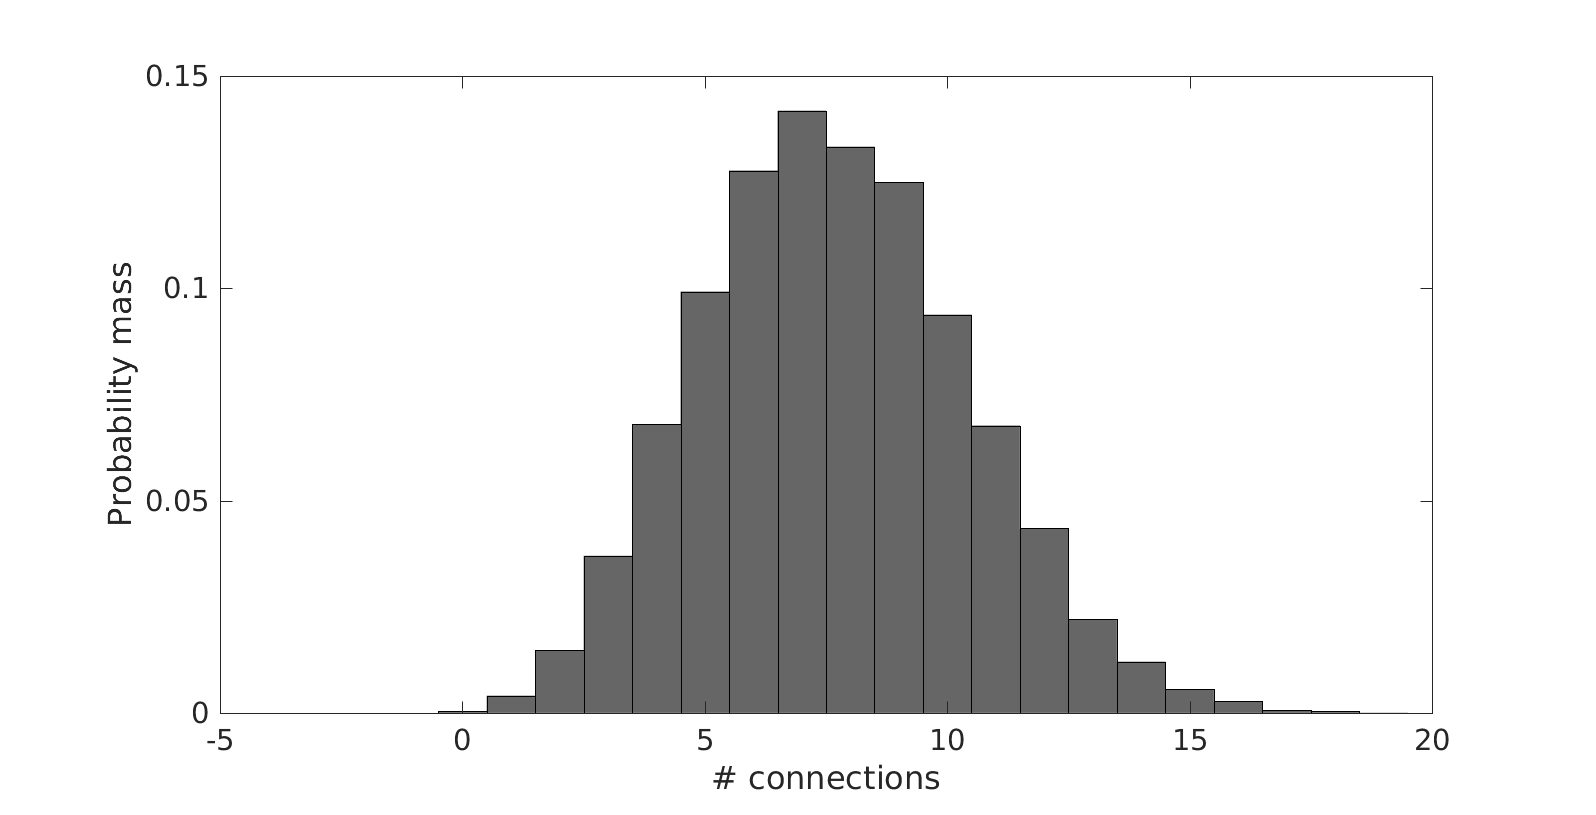
\includegraphics[width=0.6\textwidth]{fig/ConnectionNumberDistributionForest} }
     \subfloat[][]{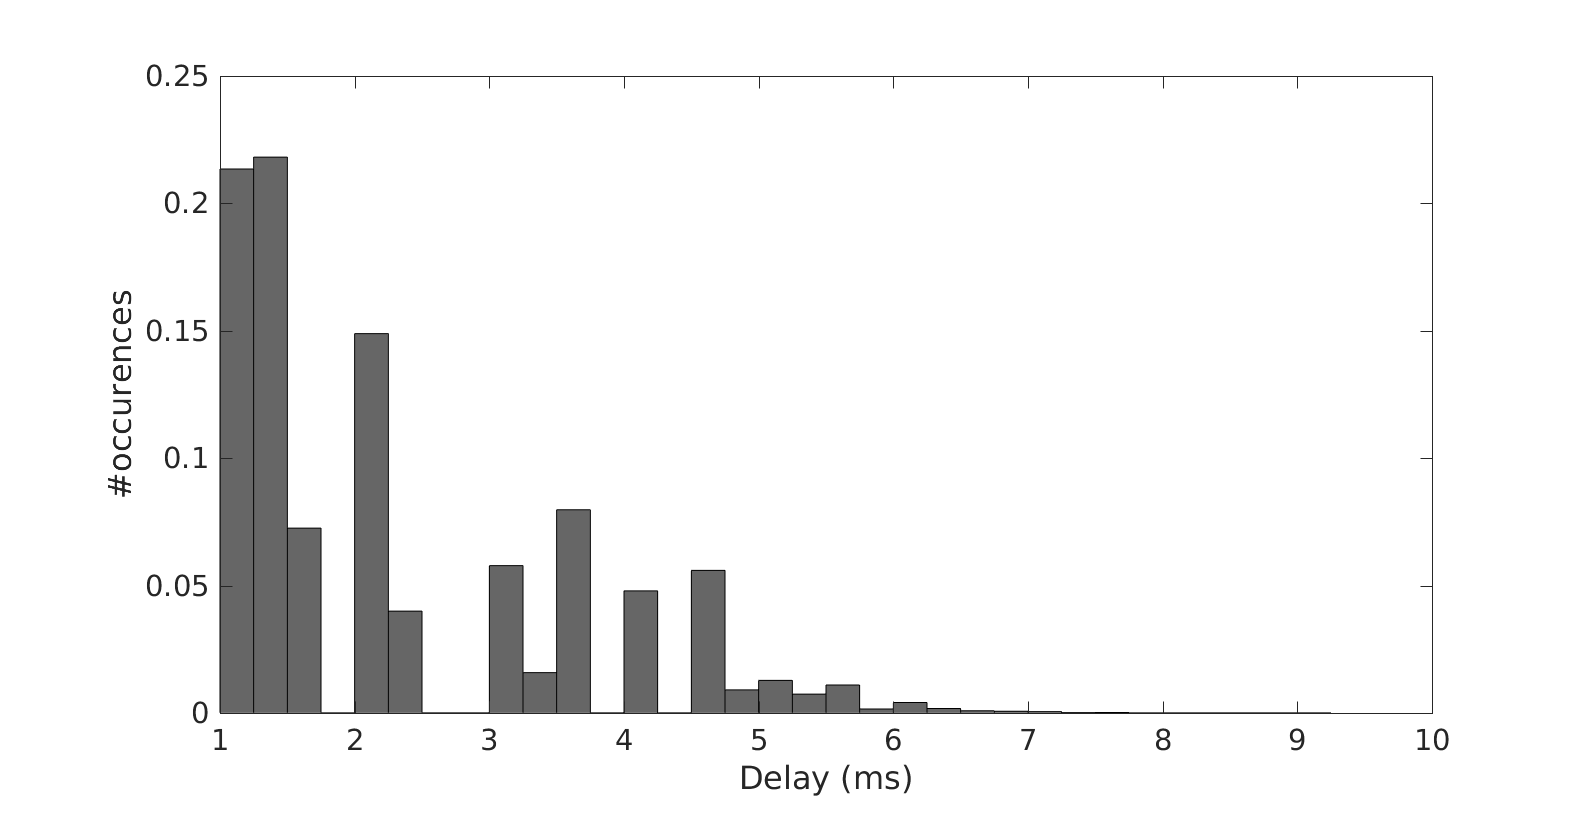
\includegraphics[width=0.6\textwidth]{fig/DelayDistributionForest} }
 \label{fig:connection_delay_distrbution_forest}
\end{figure}
 \FloatBarrier

We stimulate the forest with a uniform background stimulus. 
With $M=5$ there are many competing waves resulting in small-scale waves with many collisions.
We decrease M to 2 and increase K from 10 to 14.
We then observe traveling wave patterns in the forest.
\begin{figure}[!htb]
 \caption{ Raster plots from a forest of minicolumns with uniform background stimulus.}
   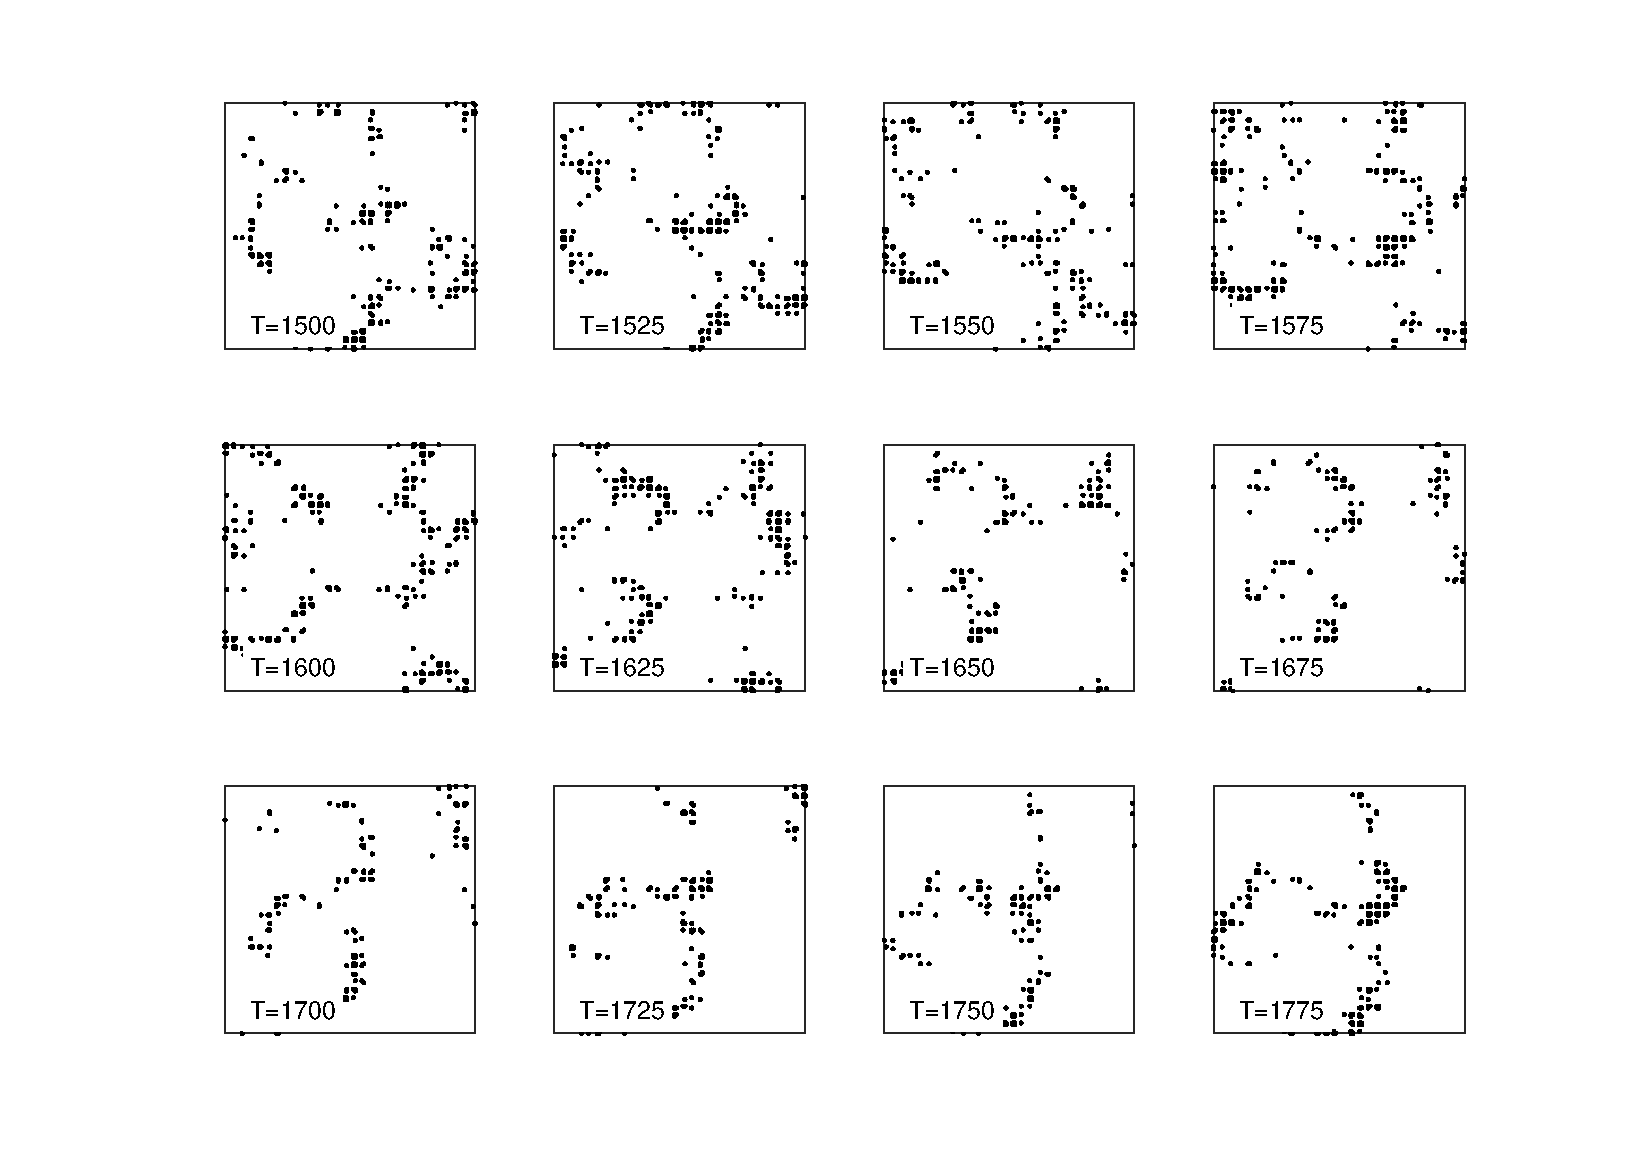
\includegraphics[width=\textwidth]{fig/ForestWaveRaster_Background_K14_M2}
   \label{fig:ForestBackground}
\end{figure}

We perform individual wave trials as in section \ref{sub:propagation_speed}.
In this case stimulate the minicolumn at X={0,1}. Y={0,1}.
We stimulate the first two layers Z={1,2}.
We observe a single wave traversing the forest in Figure \ref{fig:2_5D_Wave}.
\begin{figure}[!htb]
 \caption{ Raster plots from a forest of minicolumns looking down on the X/Y plane. 
           The 2x2 minicolumn in the lower left corner was stimulated at time $t=10\ ms$.}
   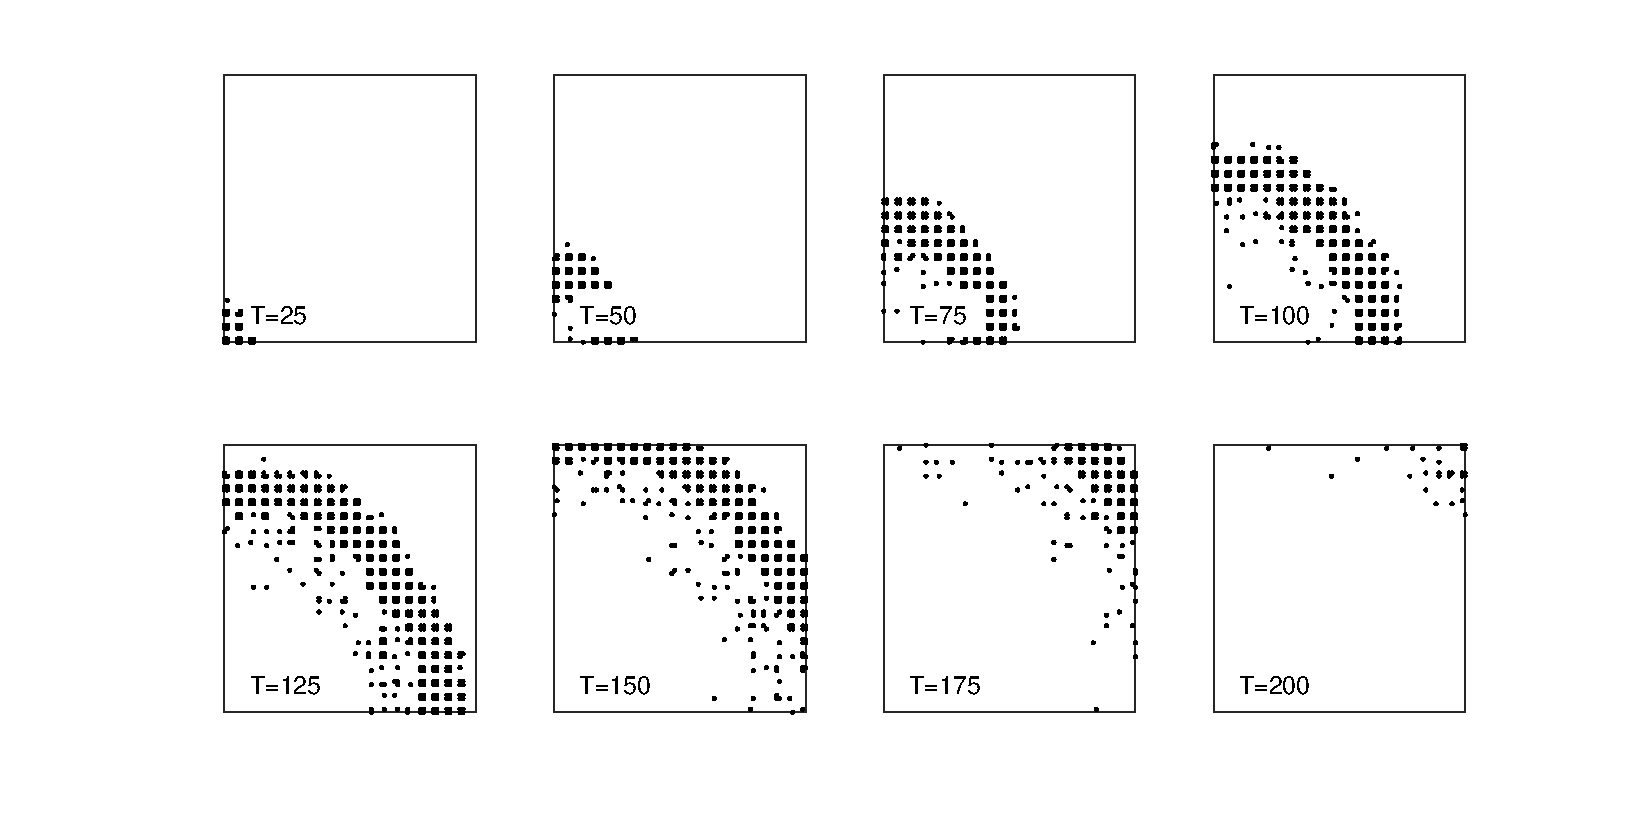
\includegraphics[width=\textwidth]{fig/Rasters_2_5D_Wave}
   \label{fig:2_5D_Wave}
\end{figure}


\FloatBarrier


\endinput
%%
%% End of file `example-1.tex'.
